\section{RQ2: Can Users See the Change?}\label{sec:rq2}

An approval is informed only if a change that matters shows up somewhere the user or client looks. In MCP, the place that matters is the tool description: it is what the model reads and what clients display. We therefore ask, for each capability gain, whether the gaining tool's description changed in the same release and whether the new text mentions the capability.

\paragraph{Tool descriptions}
Figure~\ref{fig:disclosure} shows the result. Of the 5,740 tool-level capability gains, 4,244 (73.9\%) happen while the tool's description stays byte-identical. In 1,143 (19.9\%) the description changes but says nothing about the new capability, and in only 168 (2.9\%) does the new text mention it.\footnote{The remaining 185 gains belong to tools whose descriptions are computed at run time and cannot be compared.} For high-risk classes (running commands, dynamic code, writing files, and reading secrets) the picture is the same: of 3,821 gains, 2,910 (76.2\%) are silent, 719 (18.8\%) come with an unrelated description change, and 80 (2.1\%) are disclosed. Our test for ``mentions the capability'' is a permissive keyword match, so 2.1\% is if anything an overestimate.

\begin{figure}[t]
\centering
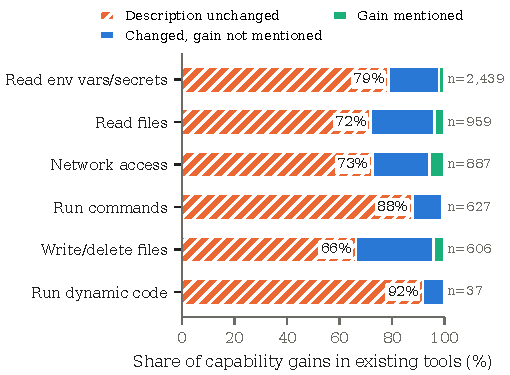
\includegraphics[width=\columnwidth]{figures/fig_disclosure.pdf}
\caption{How capability gains in existing tools appear in the tool's description, by capability class. Gains in tools with run-time descriptions are excluded.}
\label{fig:disclosure}
\end{figure}

In terms of servers, 356 (13.9\%) have at least one silent capability gain and 282 (11.0\%) a silent high-risk gain. For 53 servers (2.1\%) the silent high-risk gain sits in the tool's own handler rather than in a helper it calls, which our validation finds to be the most reliable signal (Section~\ref{sec:validation}).

\paragraph{Anything visible at all}
A user might notice a change elsewhere: a new tool, an edited description of another tool, or a changed README. We call a server-level capability gain \emph{fully silent} if none of these happens in the same release. 123 servers (4.8\%) have at least one fully silent gain, and 90 (3.5\%) a fully silent high-risk gain: the code can do something new and dangerous, and nothing a user could read has changed.

\paragraph{Self-declared annotations}
MCP lets a server declare per-tool hints such as \texttt{readOnlyHint}, a machine-readable statement a client could use instead of prose. At their latest version, 526 servers (20.5\%) declare hints on 16,341 of 85,526 tools (19.1\%), and 8,923 tools declare themselves read-only. Hints, however, do not move with the code. Of 548 high-risk capability gains in tools that carry hints, 527 (96.2\%) leave the hints unchanged. In 45 cases a tool that declared \texttt{readOnlyHint: true} gained the ability to write files, run commands, or evaluate code; in 43 it still declared itself read-only afterwards. The two exceptions show the mechanism working as intended, for example a PDF tool whose read-only flag was cleared in the release that made it write files. A hint describes an effect and our capabilities describe mechanisms, so a read-only tool that runs \texttt{ping} or writes a temporary file is not necessarily mislabelled; but a hint that is never revisited when the code changes cannot serve as the basis for approval either.

\paragraph{Instruction-like text}
Prior attacks hide instructions in descriptions, for example with invisible Unicode tag characters~\cite{unicodetag2026}. We searched every description change for such content. 209 servers (8.1\%) add text that matches at least one instruction-like pattern. We read every match for concealment or hidden characters (14 servers) and the description changes in our validation sample; all were ordinary usage directions to the model (``call \texttt{search} first; do not list every item''), not hidden instructions. A single server, out of 2,571, added a zero-width character, and it was harmless. Hidden description text is not how real servers change; code is.

\begin{finding}{2}
Users cannot see most changes. Three in four capability gains leave the tool's description untouched, only about 2\% of high-risk gains are mentioned in the text users approved, and machine-readable annotations are updated in fewer than 4\% of high-risk gains.
\end{finding}
